\newcommand{\req}[1]{RQ#1}
\begin{table}[t]
%  \vspace{2mm}
  \caption{Analysis results of NativeFlowBench}
  \label{table:RQ1-1}
  \vspace*{-1em}
  \centering
%  \footnotesize
\renewcommand{\arraystretch}{.9}
  \begin{tabular}{l||c|c}
\multicolumn{1}{c||}{\textbf{Benchmark}} & \textbf{\jnsaf} & \textbf{\ours}\\\hline\hline
    icc\_javatonative                   & $\bigcirc$ & $\times$\\
    icc\_nativetojava                   & $\bigcirc$ & $\times$\\
    native\_complexdata                 & $\bigcirc$ & $\bigcirc$\\
    native\_complexdata\_stringop       & $\times$ & $\times$\\
    native\_dynamic\_register\_multiple & $\bigcirc$ & $\bigcirc$\\
    native\_heap\_modify                & $\bigcirc$ & $\bigcirc$\\
    native\_leak                        & $\bigcirc$ & $\bigcirc$\\
    native\_leak\_array                 & $\bigcirc$ & $\times$\\
    native\_leak\_dynamic\_register     & $\bigcirc$ & $\bigcirc$\\
    native\_method\_overloading         & $\bigcirc$ & $\bigcirc$\\
    native\_multiple\_interactions      & $\bigcirc$ & $\bigcirc$\\
    native\_multiple\_libraries         & $\bigcirc$ & $\bigcirc$\\
 native\_noleak                       & $\bigcirc$ & $\bigcirc$ \\
 native\_noleak\_array                & $\times$ & $\bigcirc$  \\
 native\_nosource                     & $\bigcirc$ & $\bigcirc$  \\
 native\_pure                         & $\bigcirc$ & $\bigcirc$  \\
 native\_pure\_direct                 & $\bigcirc$ & $\bigcirc$  \\
 native\_pure\_direct\_customized     & $\bigcirc$ & $\bigcirc$  \\
 native\_set\_field\_from\_arg        & $\bigcirc$ & $\bigcirc$  \\
 native\_set\_field\_from\_arg\_field & $\bigcirc$ & $\bigcirc$  \\
 native\_set\_field\_from\_native     & $\bigcirc$ & $\bigcirc$  \\
 native\_source                       & $\bigcirc$ & $\bigcirc$  \\
 native\_source\_clean                & $\bigcirc$ & $\bigcirc$
  \end{tabular}
\vspace*{-1em}
\end{table}



\section{Evaluation}\label{sec:eval}

To show the effectiveness of our approach, we evaluate our analyzer
\ours with the following two research questions:
\begin{itemize}
  \item \textbf{\req{1}: Feasibility.} Can \ours correctly analyze multilingual
    programs that use various interoperations?

  \item \textbf{\req{2}: Usefulness.} Can \ours detect the dataflow related
    bugs that the state-of-the-art multilingual program analyzers can detect?
\end{itemize}

For \req{1}, we perform dataflow analysis on four benchmark suites using \ours.
Two benchmark suites are for Java-C program analysis. 
The first benchmark suite is NativeFlowBench~\cite{nativeflowbench, JN-SAF}
which contains 23 JNI Android applications (apps) that use various JNI
interoperations and sensitive data leakage from {\it sources} to {\it sinks}
across language boundaries via the JNI interoperations.  We compare the analysis
results of \ours to the results of the state-of-the-art Java-C program
analyzers, JN-Sum~\cite{LeeASE20} and JN-SAF~\cite{JN-SAF}. We use compiled
versions of the benchmarks for JN-SAF because it targets compiled JNI programs
and uses the source code of the benchmarks for \ours and JN-Sum.  The second
benchmark suite consists of real-world Java-C Android apps downloaded from
F-Droid, a repository of open-source Android apps~\cite{fdroid}.  We first
classified F-Droid apps into Java-C and non-Java-C apps. Then, we selected all 42
apps that can be compiled without any errors as our analysis targets.

The other two benchmark suites are for Python-C program analysis.  
The first benchmark suite is ExtModuleFlowBench we developed, which contains 20
Python-C programs.
We converted each Java-C benchmark in the NativeFlowBench into a Python-C
program, except for 8 apps containing JNI-specific interoperation
features, and made additional 5 Python-C programs that contain Python
Extension Module specific interoperations.
The second benchmark suite consists of six real-world Python-C programs
collected from public github repositories, which are analysis targets in the
previous work~\cite{cpython}.

%For \req{1}, we perform dataflow analysis on four benchmark suitess using \ours.
%Two benchmark suites are for JNI programs.
%The first benchmark suite is NativeFlowBench~\cite{nativeflowbench, JN-SAF} which is
%created by authors of JN-SAF for benchmarking for dataflow analysis of JNI
%programs. It contains 23 JNI Android applications (apps) that use various JNI
%interoperations and sensitive data leakage from {\it sources} to {\it sinks}
%across language boundaries via the interoperations.  We compare the analysis
%results of \ours to the results of JN-Sum and JN-SAF. We use compiled versions
%of the benchmarks for JN-SAF because it targets compiled JNI programs and uses
%the source code of the benchmarks for \ours and JN-Sum.
%The second benchmark suite consists of real-world JNI Android apps downloaded from
%F-Droid, a repository of open-source Android apps~\cite{fdroid}.  We first
%classified F-Droid apps into JNI and non-JNI apps. Then, we selected all 42
%apps that can be compiled without any errors as our analysis targets.

%Another two benchmark suites are for extension module programs.  The first
%benchmark suite is ExtModuleFlowBench which contains 20 extension moudle
%programs. We created this benchmark suite by referring to NativeFlowBench. We
%converted each app in NativeFlowBench into corresponding extension module
%programs, except for the apps that contains JNI-Specific interoperation
%features. Instead, programs that reflect the extension
%module-specific interoperations are added to ExtModuleFlowBench.  Similar to
%NativeFlowBench, the programs contains various forms of dataflow from
%hypothetical {\it sources} to {\it sinks} across language boundary.
%The second benchmark suite consists of 6 public github repositories that
%implement extension modules.  Each repository consists of the library that is
%written in C, and test codes that are written in Python. The test codes
%import the library code and simply call various functions in C. The benchmark is
%selected referring to the existing mulitilingual analyzer for C and
%python~\cite{}. The target analysis here is to find the possible python
%object values that can flow into the arguments of specific API function calls in C.

For \req{2}, we detect JNI interoperation bugs in the 42 real-world Android
apps using \ours. 
We implemented a checker detecting four kinds of bugs on top of \ours using the
query language of CodeQL. We chose our target JNI interoperation bugs as the
same as the targets of the client analysis of the previous
research~\cite{LeeASE20, ILEA}.
% Mention reason for not using python? (benchmark = lib-testcode => no place for bug)

\subsection{\req{1}: Feasibility}
\textbf{NativeFlowBench.} Table~\ref{table:RQ1-1} summarizes the analysis
results of \ours and \jnsaf on 23 benchmarks in NativeFlowBench.
The {\bf Benchmark} columns show the benchmark names, and the {\bf Dataflow} columns show
the analysis results of JN-SAF and \ours.
We marked each analysis result as a success ($\bigcirc$) or failure ($\times$).
An analysis succeeds if it reports all data leakages correctly without any
false positives or negatives.

\ours found data leakages correctly in 20 benchmarks but reported false
negatives for three benchmarks, while JN-SAF analyzes 21 benchmarks correctly. 
The one common failure comes from string concatenation.
{\it native\_complexdata\_stringop} generates a Java field name by
concatenating two string values via the {\tt strcat} built-in function.
Because \ours does not handle such built-in function, it failed to analyze
the benchmark.
{\it icc\_javatonative} and {\it icc\_nativetojava} leak data via the Android
inter-component communication that is beyond the scope of \ours.
The remaining two different failures of \ours and JN-SAF come from their array
analysis policies.
{\it native\_leak\_array} stores sensitive data in an array, retrieves the data
from the array, and leaks it.  
On the other hand, {\it native\_noleak\_array} stores sensitive data in an
array as well, but it retrieves another element from the array and uses it.
Because analyzing different indices of an array is challenging, JN-SAF tracks
every value retrieved from an array if the array contains sensitive data.
Such over-approximation enables JN-SAF to analyze {\it native\_leak\_array}
correctly but introduces a false alarm for {\it native\_noleak\_array}.  
In contrast, because CodeQL does not track dataflows on arrays, \ours does not
report a false alarm for {\it native\_noleak\_array} but cannot find the
leakage in {\it native\_leak\_array}.

%In the dataflow comparison, \ours found data leakages correctly in 20
%benchmarks but reported false negatives for three benchmarks, while JN-SAF
%analyzes 21 benchmarks correctly. 
%The one common failure comes from string concatenation.
%{\it native\_complexdata\_stringop} generates
%a Java field name by concatenating two string values via the {\tt strcat} built-in function.
%Because \ours and JN-Sum do not handle such built-in
%function, they failed to analyze the benchmark.
%{\it icc\_javatonative} and {\it icc\_nativetojava} leak data via the Android
%inter-component communication that is beyond the scope of \ours.
%The remaining two different failures of \ours and JN-SAF come from their array analysis policies.
%{\it native\_leak\_array} stores sensitive data in an array, retrieves the data from the array,
%and leaks it.  On the other hand, {\it native\_noleak\_array} stores sensitive
%data in an array as well, but it retrieves another element from the array and uses it.
%Because analyzing different indices of an array is challenging, JN-SAF
%tracks every value retrieved from an array if the array contains sensitive data.
%Such over-approximation enables JN-SAF to analyze {\it
%native\_leak\_array} correctly but introduces a false alarm for {\it
%native\_noleak\_array}.  In contrast, because CodeQL does not
%track dataflows on arrays, \ours does not report
%a false alarm for {\it native\_noleak\_array} but cannot find the leakage in {\it
%native\_leak\_array}.

%In the precision comparison, \ours successfully analyzed 21 out of 23
%benchmarks, while JN-Sum failed in three more benchmarks than \ours.
%We manually confirmed that the two failures both in \lees and \ours
%come from built-in structs and functions in C; {\it
%icc\_javatonative} stores Java class information in the Android built-in
%struct {\tt android\_app} and {\it native\_complexdata\_stringop} generates
%a Java field name by concatenating two string values via the {\tt strcat} built-in function.
%  Because \ours and JN-Sum do not handle such built-in
%structs and functions, they failed to analyze the two benchmarks.
%  \lees failed to analyze three more benchmarks due to native entry points
%of the benchmarks~\cite{nativeactivity}.
%  FlowDroid~\cite{Flowdroid} used by JN-Sum performs a whole-program
%analysis from Android entry points. 
%  Because the benchmarks have entry points only in C differently from monolingual
%Android apps, FlowDroid cannot find entries from which its analysis starts.
%  Contrary to JN-Sum, \ours performs a query-based
%analysis, which can resolve the targets of foreign function calls regardless of program entries.

\begin{table*}[t]
%  \vspace{2mm}
  \caption{Analysis results of real-world Android JNI applications}
  \label{table:RQ1-2}
  \vspace*{-.5em}
  \centering
  \footnotesize
%\renewcommand{\arraystretch}{.9}
  \begin{tabular}{@{}l||r|r|r|r|r||r|r|r||r|r|r@{}}
    \multirow{3}{*}{\textbf{Application}} & \multicolumn{5}{c||}{\textbf{Time (sec.)}} & \multicolumn{3}{c||}{\multirow{2}{*}{\textbf{C->Java Function Call}}} & \multicolumn{3}{c}{\multirow{2}{*}{\textbf{C->Java Field Access}}} \\\hhline{~||-----||~~~||~~~}
    & \multicolumn{3}{c|}{\textbf{DB Creation}} & \multicolumn{1}{c|}{\multirow{2}{*}{\textbf{Query}}} & \multicolumn{1}{c||}{\multirow{2}{*}{\textbf{Total}}} & \multicolumn{3}{c||}{} & \multicolumn{3}{c}{} \\\hhline{~||---~|~||------}
    & \multicolumn{1}{c|}{\textbf{C}} & \multicolumn{1}{c|}{\textbf{Java}} & \multicolumn{1}{c|}{\textbf{Merged}} & \multicolumn{1}{c|}{} & \multicolumn{1}{c||}{} & \multicolumn{1}{c|}{\textbf{\# Precise}} & \multicolumn{1}{c|}{\textbf{\# Resolved}} & \multicolumn{1}{c||}{\textbf{Total}} & \multicolumn{1}{c|}{\textbf{\# Precise}} & \multicolumn{1}{c|}{\textbf{\# Resolved}} & \multicolumn{1}{l}{\textbf{Total}}  \\\hhline{=#*{4}{=|}=#=|=|=#=|=|=}
  1. Agram                  & 2.538                 & 5.002                    & 3.643                      & 6.829                                      & 18.012                                  & 0                           & 0                            & 2                         & 4                           & 4                            & 4                          \\
  2. AndIodine              & 2.805                 & 8.237                    & 3.989                      & 8.114                                      & 23.145                                  & 1                           & 1                            & 1                         & 0                           & 0                            & 0                          \\
  3. APV PDF Viewer         & 56.496                & 9.252                    & 23.349                     & 35.688                                     & 124.785                                 & 4                           & 4                            & 4                         & 15                          & 15                           & 16                         \\
  4. CommonsLab             & 23.176                & 24.139                   & 14.149                     & 20.554                                     & 82.018                                  & 4                           & 5                            & 5                         & 0                           & 0                            & 0                          \\
  5. CrossWords             & 29.754                & 21.663                   & 23.276                     & 29.106                                     & 103.799                                 & 68                          & 68                           & 70                        & 9                           & 10                           & 14                         \\
  6. Document Viewer        & 180.71                & 20.292                   & 56.743                     & 75.934                                     & 333.679                                 & 6                           & 6                            & 6                         & 23                          & 23                           & 24                         \\
  7. DroidZebra             & 17.774                & 7.141                    & 5.817                      & 12.608                                     & 43.34                                   & 4                           & 5                            & 5                         & 0                           & 0                            & 0                          \\
  8. FBReader               & 85.398                & 27.114                   & 36.36                      & 30.072                                     & 178.944                                 & 0                           & 0                            & 0                         & 0                           & 0                            & 1                          \\
  9. Fwknop2                & 11.834                & 11.488                   & 7.395                      & 10.446                                     & 41.163                                  & 0                           & 0                            & 0                         & 0                           & 13                           & 13                         \\
  10. Graph 89               & 72.609                & 8.47                     & 41.465                     & 598.645                                    & 721.189                                 & 1                           & 1                            & 1                         & 0                           & 0                            & 0                          \\
  11. Irssi ConnectBot       & 1.284                 & 12.32                    & 6.048                      & 11.196                                     & 30.848                                  & 1                           & 1                            & 1                         & 0                           & 0                            & 2                          \\
  12. Lumicall               & 40.486                & 13.102                   & 17.328                     & 27.104                                     & 98.02                                   & 4                           & 4                            & 4                         & 2                           & 2                            & 13                         \\
  13. Navit                  & 26.761                & 17.741                   & 54.751                     & 46.264                                     & 145.517                                 & 16                          & 22                           & 55                        & 0                           & 0                            & 0                          \\
  14. NetGuard               & 14.958                & 16.925                   & 9.988                      & 12.716                                     & 54.587                                  & 0                           & 9                            & 9                         & 3                           & 27                           & 27                         \\
  15. Overchan               & 1.727                 & 22.043                   & 8.772                      & 15.143                                     & 47.685                                  & 1                           & 2                            & 4                         & 0                           & 0                            & 1                          \\
  16. Plumble                & 28.501                & 12.365                   & 16.335                     & 29.253                                     & 86.454                                  & 0                           & 0                            & 0                         & 610                         & 610                          & 610                        \\
  17. PrBoom                 & 48.312                & 5.469                    & 21.601                     & 32.001                                     & 107.383                                 & 7                           & 7                            & 15                        & 0                           & 0                            & 0                          \\
  18. Rtl-sdr driver         & 18.797                & 16.984                   & 9.623                      & 11.751                                     & 57.155                                  & 2                           & 2                            & 2                         & 0                           & 0                            & 0                          \\
  19. Sipdroid               & 20.267                & 11.864                   & 10.961                     & 18.577                                     & 61.669                                  & 2                           & 2                            & 2                         & 2                           & 2                            & 16                         \\
  20. Son of Hunky Punk      & 40.266                & 14.947                   & 20.582                     & 31.102                                     & 106.897                                 & 50                          & 50                           & 52                        & 10                          & 10                           & 10                         \\
  21. Taps Of Fire           & 3.566                 & 7.521                    & 4.453                      & 8.145                                      & 23.685                                  & 0                           & 0                            & 0                         & 2                           & 2                            & 2                          \\
  22. Tileless Map           & 273.993               & 187.099                  & 118.557                    & 146.806                                    & 726.455                                 & 50                          & 58                           & 59                        & 3                           & 4                            & 5                          \\
  23. Timidity AE            & 23.417                & 11.718                   & 13.03                      & 28.452                                     & 76.617                                  & 16                          & 16                           & 16                        & 0                           & 0                            & 0                          \\
  24. Tux Paint              & 256.126               & 120.831                  & 161.906                    & 184.591                                    & 723.454                                 & 80                          & 83                           & 89                        & 4                           & 4                            & 6                          \\
  25. VotAR                  & 1.515                 & 5.189                    & 3.569                      & 6.532                                      & 16.805                                  & 1                           & 1                            & 2                         & 3                           & 3                            & 3                          \\\hhline{=#*{4}{=}=#=|=|=#=|=|=}
    \textbf{Total}       & \multicolumn{1}{r}{}  & \multicolumn{1}{r}{}     & \multicolumn{1}{r}{}       & \multicolumn{1}{r}{}                       & \multicolumn{1}{r||}{}                    & 318                         & 347                          & 404                       & 690                         & 729                          & 767
  \end{tabular}
\end{table*}


\textbf{Real-world Java-C Programs.} Table~\ref{table:RQ1-2} summarizes the
analysis results of \ours on real-world Android Java-C apps.
Out of 42 apps we analyzed, we show the analysis results of 25 apps that have
interoperations from C to Java\footnote{We report the full analysis results in
our supplementary material.}.
The first column shows app names, the second to the fourth columns show
database creation time of C, Java, and their merged database, respectively, the
fifth shows query processing time, and the sixth shows the total analysis time.
{\bf C->Java Function Call} and {\bf C->Java Field Access} show the numbers of
C-to-Java function calls and C-to-Java field accesses, respectively. We
collectively call them \emph{JNI uses}.
The sub-columns {\bf \#Precise}, {\bf \#Resolved}, and {\bf Total} represent
the numbers of precisely resolved, resolved, and the total JNI uses,
respectively.
We considered a resolved JNI use as precise, when \ours finds a single target
method or a single field at the JNI use.


\ours resolved 1,076 out of 1,171 (92\%) JNI uses, including 347 out of 404
(86\%) C-to-Java function calls and 729 out of 767 (95\%) C-to-Java field
accesses. 
In addition, 1,008 (86\%) resolved JNI uses are precise.
The results show that \ours resolves more JNI uses even precisely than \lees. 
\lees failed to analyze one app because of an error, four apps due to the lack
of memory spaces, and three apps even in eight hours.  
In addition, \lees resolved 71\% and precisely resolved 46\% of JNI uses in the
remaining 17 apps, which shows significantly imprecise results than \ours.
%
% The results
% show that \ours resolves more JNI uses even precisley than JN-Sum. JN-Sum
% failed to analyze \inred{1} apps because of an error, \inred{4} apps because of
% lacks of memory spaces, and \inred{3} apps even in \inred{8} hours.  In
% addition, JN-Sum resolved 71\% and precisely resolved 46\% out of JNI uses in
% the remaining \inred{17} apps, which shows significantly imprecise results
% than \ours.
\ours failed to resolve 95 (8\%) JNI uses because of complex language semantics
such as arrays and function pointers.  
Because CodeQL does not track dataflows on C function pointers and arrays,
\ours failed to analyze method or field IDs necessary to resolve the JNI uses.


%\begin{figure}[t]
%  \centering
%  \vspace{2mm}
%  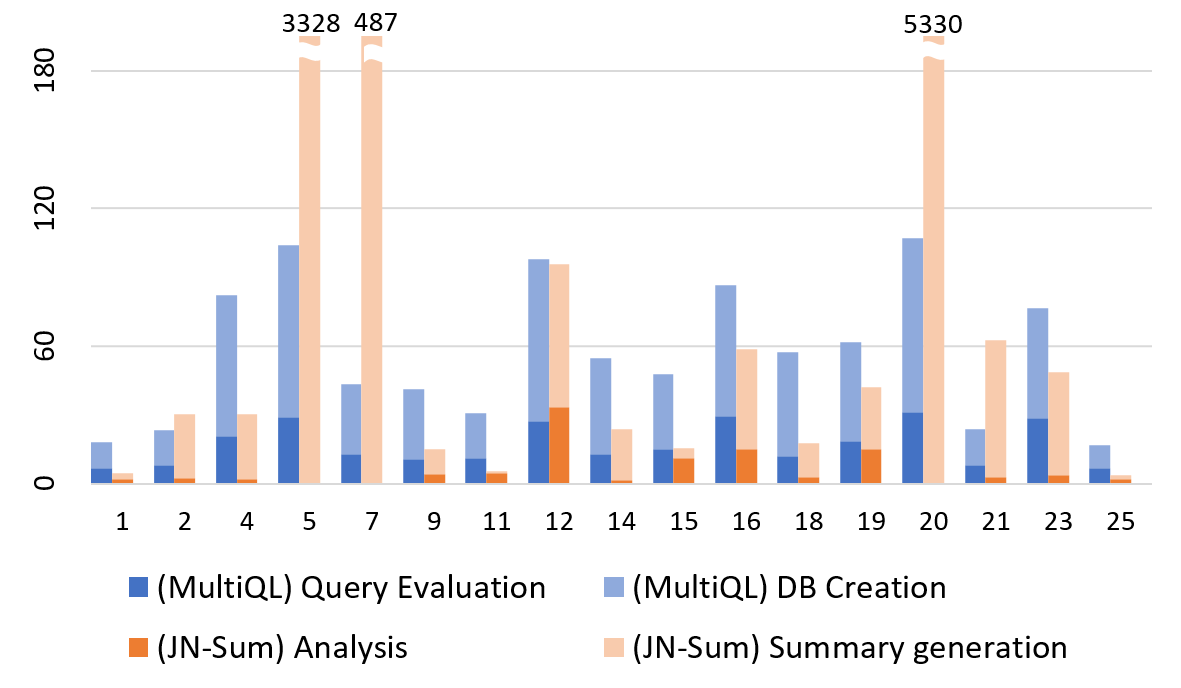
\includegraphics[width=0.47\textwidth]{img/graph}
%  \vspace*{-.5em}
%  \caption{Analysis time of \ours and \lees}
%  \label{fig:graph}
%\vspace*{-1em}
%\end{figure}

\ours is scalable in that it can analyze large-scale programs. 
The analysis time was 161.3 seconds on average for each app, including 103.8
seconds for DB creation and 57.5 seconds for query processing.  
DB creation took more time than query processing except for {\it Graph 89}, and
the DB creation time was almost linear to the code size. 
\ours took about 12 minutes at most to analyze {\it Tileless Map} having about
one million lines of code.
Note that once we create a database for a program, we can evaluate multiple
queries on it without re-creation to obtain various analysis results of the
program.
%   Note that once we
% create a database for a program, we can evaluate multiple queries on it without
% re-creation to obtain various analysis results of the program.

\begin{figure}[t]
  \centering
  \vspace{2mm}
  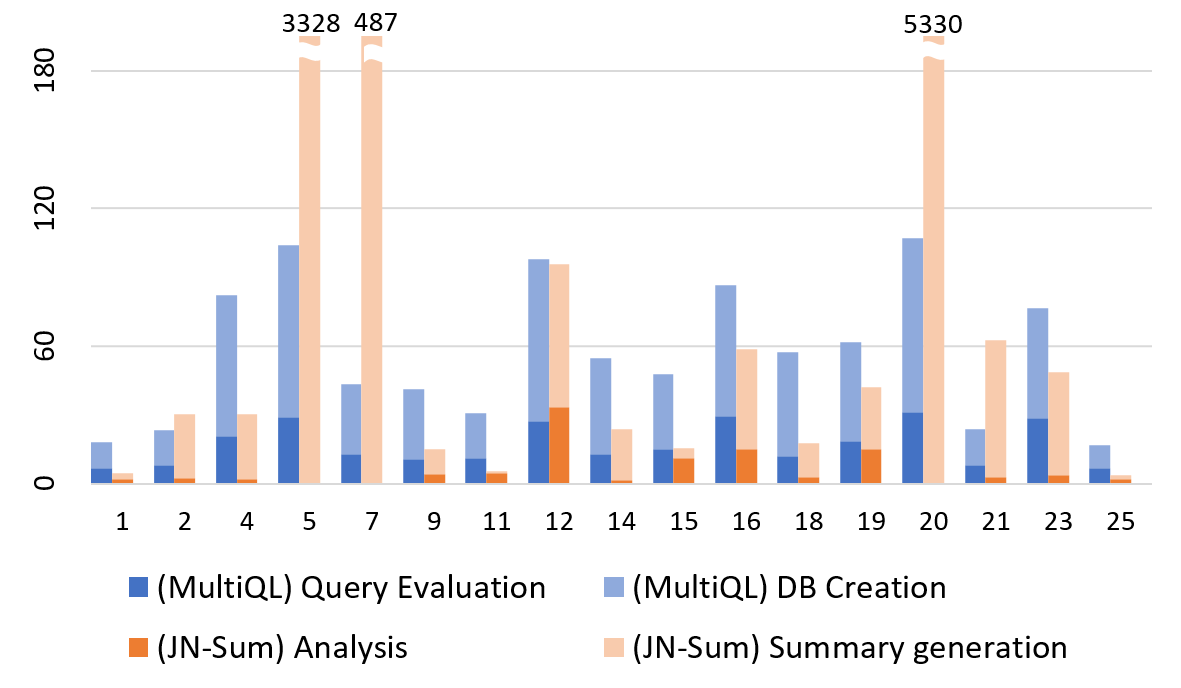
\includegraphics[width=0.47\textwidth]{img/graph}
  \vspace*{-.5em}
  \caption{Analysis time of \ours and \lees}
  \label{fig:graph}
\vspace*{-1em}
\end{figure}

%\inred{(Maybe we don't need this paragraph?)}
Figure~\ref{fig:graph} shows the analysis time of \ours compared to \lees.
The x-axis denotes the labels of apps and the y-axis denotes the analysis time
in seconds. We omit eight apps \lees failed to analyze.
\lees analyzed 12 apps faster than \ours, but the difference is less than two
minutes. 
On the other hand, \ours analyzed five apps faster than \lees, and \lees took
much time in summary generation for three apps of them. 
In addition, while \lees failed to analyze all the large-scale apps that have
more than about 400,000 lines of code in eight hours, \ours analyzed about
three million lines of code in about ten minutes.

% Figure~\ref{fig:graph} shows the analysis time of \ours compared to
% JN-Sum. Out of \inred{17} apps except for \inred{8} apps JN-Sum failed to
% analyze, JN-Sum analyzed \inred{12} apps faster than \ours. JN-Sum took about
% \inred{32} seconds on average to analyze each of them and \ours took and \ours
% was about \inred{56} seconds.  On the other hand, \ours analyzed \inred{5} apps
% faster than JN-Sum. The average analysis time of JN-Sum was about \inred{30}
% minutes, but ours was about just \inred{1} minutes. While JN-Sum usually
% analyzed small size apps faster than \ours but it took lots of time in the
% summary generation phase for some large size apps, the analysis time of \ours
% is almost linear to the size of apps.  In addition, JN-Sum failed to analyze
% all the large size apps that have more than about 400,000 lines of code in
% eight hours. Different from JN-Sum, \ours analyzed huge apps that have about
% three million lines of code in about ten minutes.

\begin{table}[t]
%  \vspace{2mm}
  \caption{Analysis results of ExtModuleFlowBench}
  \label{table:RQ1-3}
  \vspace*{-1em}
  \centering
%  \footnotesize
\renewcommand{\arraystretch}{.9}
  \begin{tabular}{l|c||l|c}
    \textbf{Benchmark} & \textbf{Dataflow} & \textbf{Benchmark} & \textbf{Dataflow}
%\\\hline\hline
\\\hhline{=|=#=|=}
    callback                    & \cmark & multiple\_module             & \cmark \\
    cobject\_member             & \cmark & noleak                       & \cmark \\
    cobject\_method             & \cmark & noleak\_array                & \cmark \\
    complexdata                 & \cmark & nosource                     & \cmark \\
    complexdata\_stringop       & \xmark & parse\_arg                   & \cmark \\
    heap\_modify                & \cmark & set\_field\_from\_arg        & \xmark \\
    import\_module              & \cmark & set\_field\_from\_arg\_field & \xmark \\
    leak                        & \cmark & set\_field\_from\_native     & \xmark \\
    leak\_array                 & \xmark & source                       & \cmark \\
    multiple\_interactions      & \cmark & source\_clean                & \xmark
  \end{tabular}
\end{table}


\textbf{ExtModuleFlowBench}
Table~\ref{table:RQ1-3} summarizes the analysis results on 20 Python-C programs
in ExtModuleFlowBench.
The {\bf Benchmark} columns show the benchmark names, and {\bf Dataflow}
columns show the analysis results of \ours.
The analysis succeeds if it reports all dataflows from {\it source} to {\it
sink} without any false positives or negatives.
\ours tracked dataflows correctly in 14 benchmarks, but reported false
negatives for six benchmarks.
\ours failed in {\it complexdata\_stringop} and {\it leak\_array} due to the
same reason in the NativeFlowBench result. 
In the other four benchmarks, \ours failed to track dataflows for fields of
Python objects. 
The benchmarks change values of fields of Python objects in C code. 
Because \ours does not handle such Python object modifications in C code, it
reported false negatives in the benchmarks.


%Table~\ref{table:RQ1-3} summarizes the analysis results of \ours.
%The {\bf Benchmark} columns show the benchmark names,
%and {\bf Dataflow} columns show the analysis results of \ours.
%The analysis succeeds if it reports all dataflow from {\it source} to {\it sink} without any false positives or negatives.
%The dataflow is analyzed correctly in 14
%benchmarks but failures were reported for six benchmarks.
%Among six failures two of them,
%{\it complexdata\_stringop} and {\it leak\_array},
%are already discussed in NativeFlowBench section.
%Additional four failures, {\it set\_field\_from*} and {\it source\_clean}
%are due to use of virtual args. In these benchmarks, a python object is
%passed to a C function as an argument. The C function modifies the field
%of this object, causing a side effect on the object. CodeQL dataflow library
%usually correctly handles this kind of side effect. However, the use of virtual arg model
%in these benchmarks was not properly reflected, and the modifications made in C function
%was not properly propagated to Python.

\begin{table}[t]
%  \vspace{2mm}
  \caption{Analysis results of real-world extension modules}
  \label{table:RQ1-4}
  \vspace*{-1em}
  \centering
%  \footnotesize
\renewcommand{\arraystretch}{.9}
\begin{tabular}{@{}l@{~}| %Repository
 @{~}r@{~}|@{~}r@{~}|@{~}r@{~}|@{~}r@{~}|@{~}r@{~}|@{~}r@{~}|@{~}r@{}}
\multicolumn{1}{@{}l|@{~}}{\multirow{2}{*}{\textbf{Repository}}}
 & \multicolumn{3}{@{~}c|@{~}}{\textbf{DB Creation (sec.)}}
 & \multicolumn{1}{@{~}c|@{~}}{\textbf{Query}}
 & \multicolumn{1}{@{~}c|@{~}}{\textbf{Total}}
 & \multicolumn{2}{@{~}c@{}}{\textbf{\# API calls}}
%\\\hhline{~|---~|~|--}
%\\\cline{2-4}\cline{7-8}
\\
\multicolumn{1}{@{}l|@{~}}{}
 & \multicolumn{1}{@{~}c|@{~}}{\textbf{Python}}
 & \multicolumn{1}{@{~}c|@{~}}{\textbf{C}}
 & \multicolumn{1}{@{~}c|@{~}}{\textbf{Merged}}
 & \multicolumn{1}{@{~}c|@{~}}{\textbf{(sec.)}}
 & \multicolumn{1}{@{~}c|@{~}}{\textbf{(sec.)}}
 & \multicolumn{1}{@{~}c|@{~}}{\textbf{Res.}}
 & \multicolumn{1}{c@{}}{\textbf{Total}}
% %\\\hhline{=#*{4}{=|}=#=|=}
\\\hline\hline
  % 1. bitarray           & 19.378 & 3.082 & 13.537 & 197.556 & 233.553 & 38 & 50 \\
  % 2. distance           & 16.722 & 2.354 & 11.594 & 134.895 & 165.565 & -  & -  \\
  % 3. noise              & 18.79  & 2.43  & 12.222 & 148.021 & 181.463 & -  & -  \\
  % 4. pyahocorasick      & 19.179 & 2.62  & 13.118 & 172.62  & 207.537 & 33 & 43 \\
  % 5. python-Levenshtein & 17.187 & 3.144 & 12.686 & 153.95  & 186.967 & -  & -  \\
  % 6. python-llist       & 17.047 & 2.853 & 11.986 & 153.014 & 184.9   & 18 & 30 \\\hhline{=#*{4}{=}=#=|=}
\multicolumn{1}{@{}l|@{~}}{bitarray}
           & 19.378 & 3.082 & 13.537 & 197.556 & 233.553 & 38 & 50 \\
\multicolumn{1}{@{}l|@{~}}{distance}
           & 16.722 & 2.354 & 11.594 & 134.895 & 165.565 & -  & -  \\
\multicolumn{1}{@{}l|@{~}}{noise}
            & 18.790  & 2.430  & 12.222 & 148.021 & 181.463 & -  & -  \\
\multicolumn{1}{@{}l|@{~}}{pyahocorasick}
      & 19.179 & 2.620  & 13.118 & 172.620  & 207.537 & 33 & 43 \\
\multicolumn{1}{@{}l|@{~}}{python-Levenshtein} & 17.187 & 3.144 & 12.686 & 153.950  & 186.967 & -  & -  \\
\multicolumn{1}{@{}l|@{~}}{python-llist}       & 17.047 & 2.853 & 11.986 & 153.014 & 184.900   & 18 & 30
%\\\hhline{=#*{4}{=}=#=|=}
\\\hline\hline
\multicolumn{1}{@{}l|@{~}}{\textbf{Total}}
 & \multicolumn{1}{r}{}
 & \multicolumn{1}{r}{}
 & \multicolumn{1}{r}{}
 & \multicolumn{1}{r}{}
 & \multicolumn{1}{r|@{~}}{}
 & 89                         & 123                          
  \end{tabular}
\vspace*{-1em}
\end{table}


%\textbf{Github}
\textbf{Real-world Python-C Programs.}
Table~\ref{table:RQ1-4} summarizes the dataflow analysis results on six
real-world Python-C programs. 
The first column shows repository names, the second to the fourth columns show
database creation time of Python, C, and their merged database, respectively,
the fifth shows query processing time, the sixth shows the total analysis time,
and the last column denotes analysis results.
{\bf \#Total} denotes the total number of Python Extension Module API function
calls in C code. 
%{\bf \#Resoved} denotes the number of API function calls of which the first
%argument is identified correctly. 
{\bf \#Resoved} denotes the number of resolved API function calls in C code.
Because all the API functions take a Python object as the first argument, we
counted an API function call as resolved, when \ours finds its first argument
correctly. 

%Table~\ref{table:RQ1-4} summarizes the dataflow analysis results for six public
%repositories in github that contain extension modules.  The first column shows
%repository names, the second to the fourth columns show database creation time
%of C, Java, and their merged database, respectively, the fifth shows query
%processing time, and the sixth shows the total analysis time.  The last coulmn
%denotes the analysis result if applicable. {\bf \#Total} denotes the total
%number of target API function calls. The target API functions are extension
%module API function calls where its first arguments are expected to be Python
%object.  The target functions are selected by finding function calls with
%prefix \ccode{PyObject\_}, \ccode{PyList\_}, \ccode{PyTuple\_},
%\ccode{PyDict\_}, and \ccode{PyArg\_}.  {\bf \#Resoved} denothes whether the
%analyzer could find the python object that flows into the argument of each API
%function calls.

%The analysis time is dominated by python analysis.  When CodeQL performs
%analysis for python, it creates database for every builtin libraries of python,
%and some predicates are also evaluated on this database. The improvement in
%performance of CodeQL's Python analysis would also make our extended
%multilingual analyzer run faster.

Out of the six programs, we exclude three programs from our evaluation targets.
{\it python-Levenshtein} contains both Python and C code, but the Python code only contained a class that works as a wrpper for C code without actual uses cases,
making no meaningful interaction between Python and C Code.
{\it distance} and {\it noise} contain too complicated Python code for CodeQL
to handle.

In the remaining three programs, \ours resolved 89 out of 123 (72.4\%) total
API function calls. 
It failed to resolve 34 API function calls due to implicit method calls in
Python. 
Python calls some methods implicitly, a class destructor for example, and C
code can register C functions as such methods. 
Because \ours does not handle C functions implicitly called in Python, it
failed to resolve API functions calls in the functions.


%The analysis result was applicable for three out of six benchmarks.
%One of them, {\it python-Levenshtein} did not contain the Python code that
%properly uses C code of extension module and thus the analysis was not
%applicable.
%Two of them, {\it distance} and {\it noise} were excluded due to limitation of
%CodeQL's python analysis. 
%The use pattern of imported modules in these benchmarks showed highly complex
%behavior, and CodeQL could not handle such behaviors to properly pass the value
%across modules. 
%In other words, CodeQL would not have been able to find correct dataflow, even
%if the C code is replaced with the python code with same functionality.
%For three benchmarks that were applicable, among 121 API function calls, the
%argument was resolved for 89 of them (72.4\%). 
%The reason for unresolved arguments were mainly due to C functions that are
%implicitly called. 
%For example, one can register a C function that is called when a python object
%is deallocated, but the explicit call site that call this function does not
%exist, there is not any value that flows into the parameter of this function. 
%Therefore, any API function calls insde this destructor function can not
%resolve the target.


\subsection{RQ2: Usefulness}
\begin{table*}[t]
  \vspace{2mm}
  \caption{The analysis result for F-Droid applications}
  \label{table:RQ2}
  \vspace*{-1em}
  \centering
  \small
  \begin{tabular}{l||r|r|r|r|r||r|r|r||r|r|r}
    \multirow{3}{*}{\textbf{Application}} & \multicolumn{5}{c||}{\textbf{Time (sec.)}} & \multicolumn{3}{c||}{\multirow{2}{*}{\textbf{C->Java Function Call}}} & \multicolumn{3}{c}{\multirow{2}{*}{\textbf{C->Java Field Access}}} \\\hhline{~||-----||~~~||~~~}
    & \multicolumn{3}{c|}{\textbf{DB Creation}} & \multicolumn{1}{c|}{\multirow{2}{*}{\textbf{Query}}} & \multicolumn{1}{c||}{\multirow{2}{*}{\textbf{Total}}} & \multicolumn{3}{c||}{} & \multicolumn{3}{c}{} \\\hhline{~||---~|~||------}
    & \multicolumn{1}{c|}{\textbf{C}} & \multicolumn{1}{c|}{\textbf{Java}} & \multicolumn{1}{c|}{\textbf{Merged}} & \multicolumn{1}{c|}{} & \multicolumn{1}{c||}{} & \multicolumn{1}{c|}{\textbf{\# Precise}} & \multicolumn{1}{c|}{\textbf{\# Resolved}} & \multicolumn{1}{c||}{\textbf{Total}} & \multicolumn{1}{c|}{\textbf{\# Precise}} & \multicolumn{1}{c|}{\textbf{\# Resolved}} & \multicolumn{1}{l}{\textbf{Total}}  \\\hhline{=#*{4}{=|}=#=|=|=#=|=|=}
  Agram                  & 2.538                 & 5.002                    & 3.643                      & 6.829                                      & 18.012                                  & 0                           & 0                            & 2                         & 4                           & 4                            & 4                          \\
  AndIodine              & 2.805                 & 8.237                    & 3.989                      & 8.114                                      & 23.145                                  & 1                           & 1                            & 1                         & 0                           & 0                            & 0                          \\
  APV PDF Viewer         & 56.496                & 9.252                    & 23.349                     & 35.688                                     & 124.785                                 & 4                           & 4                            & 4                         & 15                          & 15                           & 16                         \\
  CommonsLab             & 23.176                & 24.139                   & 14.149                     & 20.554                                     & 82.018                                  & 4                           & 5                            & 5                         & 0                           & 0                            & 0                          \\
  CrossWords             & 29.754                & 21.663                   & 23.276                     & 29.106                                     & 103.799                                 & 68                          & 68                           & 70                        & 9                           & 10                           & 14                         \\
  Document Viewer        & 180.71                & 20.292                   & 56.743                     & 75.934                                     & 333.679                                 & 6                           & 6                            & 6                         & 23                          & 23                           & 24                         \\
  DroidZebra             & 17.774                & 7.141                    & 5.817                      & 12.608                                     & 43.34                                   & 4                           & 5                            & 5                         & 0                           & 0                            & 0                          \\
  FBReader               & 85.398                & 27.114                   & 36.36                      & 30.072                                     & 178.944                                 & 0                           & 0                            & 0                         & 0                           & 0                            & 1                          \\
  Fwknop2                & 11.834                & 11.488                   & 7.395                      & 10.446                                     & 41.163                                  & 0                           & 0                            & 0                         & 0                           & 13                           & 13                         \\
  Graph 89               & 72.609                & 8.47                     & 41.465                     & 598.645                                    & 721.189                                 & 1                           & 1                            & 1                         & 0                           & 0                            & 0                          \\
  Irssi ConnectBot       & 1.284                 & 12.32                    & 6.048                      & 11.196                                     & 30.848                                  & 1                           & 1                            & 1                         & 0                           & 0                            & 2                          \\
  Lumicall               & 40.486                & 13.102                   & 17.328                     & 27.104                                     & 98.02                                   & 4                           & 4                            & 4                         & 2                           & 2                            & 13                         \\
  Navit                  & 26.761                & 17.741                   & 54.751                     & 46.264                                     & 145.517                                 & 16                          & 22                           & 55                        & 0                           & 0                            & 0                          \\
  NetGuard               & 14.958                & 16.925                   & 9.988                      & 12.716                                     & 54.587                                  & 0                           & 9                            & 9                         & 3                           & 27                           & 27                         \\
  Overchan               & 1.727                 & 22.043                   & 8.772                      & 15.143                                     & 47.685                                  & 1                           & 2                            & 4                         & 0                           & 0                            & 1                          \\
  Plumble                & 28.501                & 12.365                   & 16.335                     & 29.253                                     & 86.454                                  & 0                           & 0                            & 0                         & 610                         & 610                          & 610                        \\
  PrBoom                 & 48.312                & 5.469                    & 21.601                     & 32.001                                     & 107.383                                 & 7                           & 7                            & 15                        & 0                           & 0                            & 0                          \\
  Rtl-sdr driver         & 18.797                & 16.984                   & 9.623                      & 11.751                                     & 57.155                                  & 2                           & 2                            & 2                         & 0                           & 0                            & 0                          \\
  Sipdroid               & 20.267                & 11.864                   & 10.961                     & 18.577                                     & 61.669                                  & 2                           & 2                            & 2                         & 2                           & 2                            & 16                         \\
  Son of Hunky Punk      & 40.266                & 14.947                   & 20.582                     & 31.102                                     & 106.897                                 & 50                          & 50                           & 52                        & 10                          & 10                           & 10                         \\
  Taps Of Fire           & 3.566                 & 7.521                    & 4.453                      & 8.145                                      & 23.685                                  & 0                           & 0                            & 0                         & 2                           & 2                            & 2                          \\
  Tileless Map           & 273.993               & 187.099                  & 118.557                    & 146.806                                    & 726.455                                 & 50                          & 58                           & 59                        & 3                           & 4                            & 5                          \\
  Timidity AE            & 23.417                & 11.718                   & 13.03                      & 28.452                                     & 76.617                                  & 16                          & 16                           & 16                        & 0                           & 0                            & 0                          \\
  Tux Paint              & 256.126               & 120.831                  & 161.906                    & 184.591                                    & 723.454                                 & 80                          & 83                           & 89                        & 4                           & 4                            & 6                          \\
  VotAR                  & 1.515                 & 5.189                    & 3.569                      & 6.532                                      & 16.805                                  & 1                           & 1                            & 2                         & 3                           & 3                            & 3                          \\\hhline{=#*{4}{=}=#=|=|=#=|=|=}
    \textbf{Total}       & \multicolumn{1}{r}{}  & \multicolumn{1}{r}{}     & \multicolumn{1}{r}{}       & \multicolumn{1}{r}{}                       & \multicolumn{1}{r||}{}                    & 318                         & 347                          & 404                       & 690                         & 729                          & 767
  \end{tabular}
\end{table*}

The bug checker of \ours detects four kinds of JNI interoperation bugs
that previous research~\cite{ILEA, LeeASE20} defined as follows:

\begin{itemize}
  \item {\it NullDereference}: dereferencing the {\tt null} value of Java in C
  \item {\it MissingFun}: calling a missing Java method from C
  \item {\it TypeMismatch}: declaring a C function with a different signature
    from its corresponding Java native method
  \item {\it WrongSignature}: calling a Java method using a method ID with a
    wrong signature in C
\end{itemize}


\begin{figure}[t]
  \centering
  \vspace{2mm}
  \begin{subfigure}[t]{0.5\textwidth}
    \begin{lstlisting}[style=java,xleftmargin=2.5em]
//EmulatorActivity.java
String tmp = null;
String folder = Util.GetInternalAppStorage(activity);
if (folder != null) {
  tmp = folder + "tmp";
  Util.CreateDirectory(tmp);
}
EmulatorActivity.nativeInitGraph89(..., tmp);
    \end{lstlisting}
    \begin{lstlisting}[style=cpp,xleftmargin=2.5em]
//wrappercommonjni.c
void nativeInitGraph89(..., jstring tmp_dir) {
   (*env)->GetStringUTFChars(env, tmp_dir, 0); ...
}
    \end{lstlisting}
    \vspace*{-.5em}
    \caption{NullDereference}
    \label{fig:bug1}
  \end{subfigure}
  \begin{subfigure}[t]{0.5\textwidth}
    \begin{lstlisting}[style=java,xleftmargin=2.5em]
//JpegRedaction.java
package org.witness.obscuracam.photo.jpegredaction;

public class JpegRedaction {
  private native void redactRegions(...); ...
}
    \end{lstlisting}
    \begin{lstlisting}[style=cpp,xleftmargin=2.5em]
//JpegRedaction.cpp
void Java_org_witness_securesmartcam_jpegredaction_ JpegRedaction_redactRegions(...) { ... }
    \end{lstlisting}
    \vspace*{-.5em}
    \caption{MissingFun}
    \label{fig:bug2}
  \end{subfigure}
  \begin{subfigure}[t]{0.5\textwidth}
    \begin{lstlisting}[style=java,xleftmargin=2.5em]
//MuPdfPage.java
private native static List<PageTextBox> search(...);
    \end{lstlisting}
    \begin{lstlisting}[style=cpp,xleftmargin=2.5em]
//mupdfdroidbridge.c
jobjectArray search(...){ ... }
    \end{lstlisting}
    \vspace*{-.5em}
    \caption{TypeMismatch}
    \label{fig:bug3}
  \end{subfigure}
  \begin{subfigure}[t]{0.5\textwidth}
    \begin{lstlisting}[style=java,xleftmargin=2.5em]
//PrBoomActivity.java
void OnMessage(String text);
void OnInfoMessage(String msg, int displayType);
    \end{lstlisting}
    \begin{lstlisting}[style=cpp,xleftmargin=2.5em]
//jni_doom.h
#define CB_CLASS_MSG_SIG  "(Ljava/lang/String;I)V"
#define CB_CLASS_INFMSG_SIG  "(Ljava/lang/String;I)V"
//jni_doom.c
mSendStr = (*env)->GetMethodID(env, jNativesCls,
                       "OnMessage", CB_CLASS_MSG_SIG);
    \end{lstlisting}
    \vspace*{-.5em}
    \caption{WrongSignature}
    \label{fig:bug3}
  \end{subfigure}
  \vspace*{-.5em}
  \caption{Four kinds of JNI interoperation bugs}
  \label{fig:bugs}
  \vspace*{-1em}
\end{figure}

Table~\ref{table:RQ2} summarizes the bug detection results of 19 out of 42
apps, on which \ours reported possible bugs.  The first
column shows app names, the second and the third columns show the
number of true and false positives for {\it NullDereference}, respectively, and
the fourth to six columns show the number of true positives for {\it
MissingFun}, {\it TypeMismatch}, and {\it WrongSig}, respectively.
\ours did not report any false positives for the last three bug kinds.
We confirmed true and false positives by manual inspection of the source code. 

\ours found 33 genuine bugs, but reported 21 false positives in 19 apps.
All false positives are reported only in the {\it NullDereference} bug
detection; \ours reported five true and 21 false alarms of {\it
NullDereference} in 11 apps, nine true alarms of {\it MissingFun} in
three apps, 17 true alarms of {\it TypeMismatch} in eight apps, and two true
alarms of {\it WrongSignature} in two apps. We manually checked that the false
positives come from diverse over-approximation issues of static analyses, but
one of the main causes is conditionally sanitized variables.  Many apps
have a code pattern that assigns a value to a variable only if the variable has
the {\tt null} value. Because our analysis does not support the
path-sensitivity that analyzes each execution path separately, it reports that
the variable may still have {\tt null} even after the conditional assignment.
Note that \lees could not find 12 out of 33 bugs
due to memory or scalability issues.

Figure~\ref{fig:bugs} demonstrates four kinds of JNI interoperation bugs \ours
detected from real-world apps using simplified code.

Figure~\ref{fig:bugs}(a) shows a pattern in Graph 89 with the {\it NullDereference} bug.
The Java code may call a C function {\tt nativeInitGraph89} with {\tt
null} as its last argument, because the variable {\tt tmp} has {\tt
null} when the method {\tt GetInternalAppStorage} returns {\tt null}.  The C
function calls a JNI function {\tt GetStringUTFChars} with the value as its
second argument, without checking whether it is {\tt null}. However, because the JNI
specification describes that the second argument of the functions must not be
{\tt null}~\cite{getstringutfchars}, the function may behave unexpectedly.
Note that calling JNI functions with wrong arguments may introduce various
unexpected behaviors, since JVMs do not validate the arguments because of
performance overhead~\cite{hwang2021justgen}.

\renewcommand{\texttt}[1]{%
  \begingroup
  \ttfamily
  \begingroup\lccode`~=`/\lowercase{\endgroup\def~}{/\discretionary{}{}{}}%
  \begingroup\lccode`~=`[\lowercase{\endgroup\def~}{[\discretionary{}{}{}}%
  \begingroup\lccode`~=`.\lowercase{\endgroup\def~}{.\discretionary{}{}{}}%
  \catcode`/=\active\catcode`[=\active\catcode`.=\active
  \scantokens{#1\noexpand}%
  \endgroup
}

Figure~\ref{fig:bugs}(b) shows a pattern in ObscuraCam with the {\it MissingFun} bug.
As described in Section~\ref{sec:merging}, JNI has a C function
naming convention for JVMs to link Java native methods to their corresponding C
functions. While a Java class {\tt JpegRedaction} declaring a native method
{\tt redactRegions} belongs to a package
\texttt{org.witness.obscuracam.photo.jpegredaction}, the corresponding C
function is named with a wrong package name
\texttt{org.witness.securesmartcam.jpegredaction}.  When calling the native
method, JVM fails to link it because of the wrongly named C function.


Figure~\ref{fig:bugs}(c) shows a pattern in Document Viewer with the {\it TypeMismatch} bug.
While the return type of a Java native method {\tt search}
is {\tt List<PageTextBox>}, the return type of the corresponding C function
{\tt search} is {\tt jobjectArray} corresponding to the Java built-in array
container. The return type mismatch has no effect on linking between
Java native methods and C functions. However, since it is an unspecified case in
the JNI specification, interoperations via such native methods may behave
differently on different JVMs~\cite{LeeASE20}. 


Figure~\ref{fig:bugs}(d) shows a pattern in PrBoom with the {\it WrongSignature} bug.
The C code tries to get an ID of a Java method {\tt OnMessage} with a
signature \texttt{(LJava/lang/String;I)V}, but the method has a different
signature \texttt{(LJava/lang/String;)V} with one String argument. Because
the signatures do not match, the C code always receives {\tt null}
instead of a method ID, and this example throws a Java exception. In
addition, it may introduce errors in subsequent instructions when using the
return value without null checking or calling JNI functions without handling the
thrown Java exception~\cite{jniexcept}.
